\chapter{ПОСТАНОВКА ЗАДАЧИ ПОЛУЧЕНИЯ, АНАЛИЗА И ОБРАБОТКИ ЭКСПЕРТНОЙ ИНФОРМАЦИИ} \label{chapt1}

\section{Возникновение области} \label{sect1_1}
В настоящее время в области IT набрало большую популярность системы удаленной поддержки информационной инфраструктуры, так называемый «Аутсорсинг». Ввиду развития рынка компаниям становится невыгодно держать свой штат службы поддержки, и они отдают свою инфраструктуру сторонней компании.
Большинство проблем, которые решает удаленная служба поддержки носят весьма тривиальный характер.

\begin{itemize}
	\item Установить приложение
	\item Переустановить приложение
	\item Решить проблему с доступом к тому или иному ресурсу
\end{itemize}
Данные проблемы решают специалисты технической поддержки. Обычно техническая поддержка делится на несколько линий.

\begin{table} [htbp]
  \centering
  \parbox{15cm}{\caption{Описание работы специалистов различных уровней поддержки}\label{TSSDescription}}
%  \begin{center}
  \begin{tabular}{| p{7cm} || p{7cm} |}
  \hline
  \hline
Уровень & Описание \\
  \hline
    \hline

Первая линия	& Решение уже известных, задокументированных проблем, работа напрямую с пользователем \\
  \hline

Вторая линия  & Решение ранее неизвестных проблем \\
  \hline

Третья линия & Решение сложных и нетривиальных проблем \\
  \hline

Четвертая линия  & Решение архитектурных проблем инфраструктуры \\

  \hline
  \hline
  \end{tabular}
%  \end{center}
\end{table}


Каждая линия поддержки представлена специалистами. В среднем команда, обслуживающая одного заказчика насчитывает 60 человек. Процентное соотношение специалистов разных линий поддержки отображено на Диаграмме \ref{img:ITSMTeamComposition}

\begin{figure} [h] 
  \center
  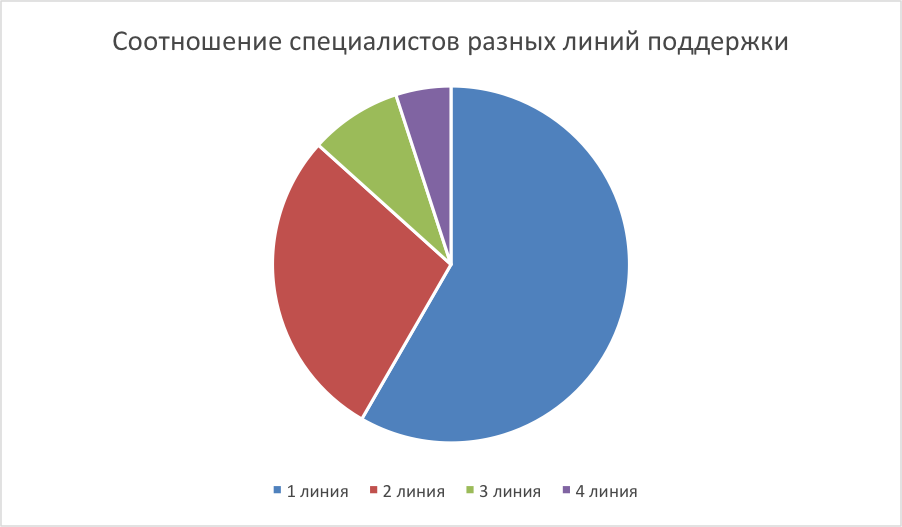
\includegraphics [scale=0.7] {ITSMTeamComposition}
  \caption{Диаграмма состава команд} 
  \label{img:ITSMTeamComposition}  
\end{figure}

Работа специалиста 1 линии поддержки состоит из множества рутинных и простых задач. На Диаграмме \ref{img:EngineerTasks}  показано соотношение разных типов проблем, встречающихся во время работы поддержки

\begin{figure} [h] 
  \center
  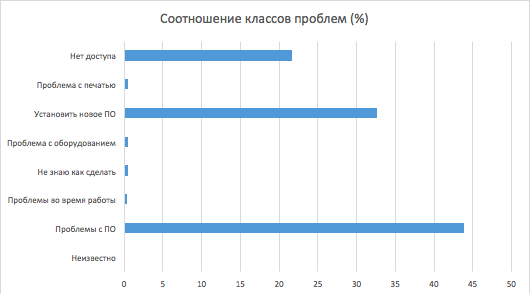
\includegraphics [scale=0.7] {EngineerTasks}
  \caption{Диаграмма соотношений типов проблем} 
  \label{img:EngineerTasks}  
\end{figure}

\begin{table} [htbp]
  \centering
  \parbox{15cm}{\caption{Категории инцидентов в области удаленной поддержки инфраструктуры}\label{IncidentDescription}}
%  \begin{center}
  \begin{tabular}{| p{7cm} || p{7cm} |}
  \hline
  \hline
Категория & Описание \\
  \hline
Проблема с ПО	& Проблема при запуске ПО на компьютере. Решается переустановкой \\
Проблемы во время работы  & Проблема с функционированием программного обеспечения\\
Как сделать & Запрос на инструкцию по работе с тем или иным компонентом рабочей станции \\
Проблема с оборудованием  & Неполадки на уровне оборудования \\
Установить новое ПО       & Требование установки нового программного обеспечения \\
Проблема с печатью        & Установка принтера в систему \\
Нет доступа               & Нет доступа к общим ресурсам \\
  \hline
  \hline
  \end{tabular}
%  \end{center}
\end{table}

Решение части задач может быть автоматизировано, а специалисты получат дополнительное время на решение более интересных задач. 
Проблема заключается в автоматизации решения рутинных задач в области удаленной поддержки инфраструктуры.

%\newpage
%============================================================================================================================

\section{Прогноз развития области} \label{sect1_2}
Основной тенденцией в развитии области удаленной поддержки инфраструктуры является попытки удешевить и улучшить стоимость предоставления услуг. \\
Компании, работающие на этом рынке вкладывают большие деньги в автоматизацию. Кроме того современное развитие науки и техники, а точнее вычислительных мощностей позволяет автоматизацию даже самых наукоемких процессов. \\
Дальнейшим развитием области является замена человеческих специалистов на автоматические системы. Многие ведущие компании ведут разработки в этом направлении. Например, компания HP. Данная компания имеет свою системы по регистрации подобных инцидентов и сейчас ведется работа над автоматизацией системы. \\

\section{Методологии, используемые в области IT аутсорсинга: ITIL и ITSM} \label{sect1_3}
В области IT аутсорсинга есть несколько готовых стандартов ведения работ. Одним из таких стандартов является библиотека ITIL. Данные стандарт описывает лучшие практики организации работ в области IT аутсорсинга. Используемый в библиотеки подход соответствует стандартам ISO 9000 (ГОСТ Р ИСО 9000) .
Наличие стандартов в области диктует унифицированность постановки проблем, а также унифицированность алгоритмов решения. Такие предпосылки говорят о возможности частично или в некоторых случаях полной автоматизации решения проблем.
\section{Постановка задачи} \label{sect1_4}
Задачами данного исследования являются:
\begin{itemize}
	\item Изучение возможности автоматизации области удаленной поддержки инфраструктуры путем анализа области
	\item Выработка критериев и сравнительный анализ существующих решений в области
	\item Создание модели проблемно-ориентированной системы принятия решений для решения задача автоматизации поддержки удаленной инфраструктуры
	\item Создание проблемно-ориентированной системы принятия решений для автоматизации поддержки удаленной инфраструктуры
	\item Создание методических рекомендаций для проведения верификации, проведение верификации и представление результатов 
	\item Подсчет статистических результатов работы комплекса

\end{itemize}



\clearpage
